%Erzeuge mit pdflatex direkt pdfs statt dvi
\pdfoutput=1\relax
\pdfcompresslevel=9
%\pdfpagewidth=8.26in
%\pdfpageheight=11.69in

%&latex
% headsepline: Linie am oberen Blattrand unterhalb der Seitennummer
% bibtotoc: Aufnahme des Literaturverzeichnisses ins Inhaltsverzeichnis
\documentclass[a4paper,headsepline]{scrreprt}


% Einstellungen bez. des 'scrreprt'-Stils

% Caption Schriftstil und -Groesse
\renewcommand{\capfont}{\normalsize}
\renewcommand{\caplabelfont}{\normalsize\bfseries}

\typearea{15}  %Einstellung des Verhältnisses Größe des Textes zur Papiergröße

% Sprache
\usepackage[english]{babel}
\addto\extrasgerman{\renewcommand{\figurename}{Abb.}}
\addto\extrasgerman{\renewcommand{\tablename}{Tab.}}


% Bilder
\usepackage{graphicx}

% Bild und Tabellenunterschriften:
\usepackage{prettyref}
% für referenzen, z.B. label für section: \label{sec:abschnittslabel}verwenden
\newrefformat{eq}{\textup{(\ref{#1})}}
\newrefformat{cha}{Chapter~\ref{#1}}
\newrefformat{sec}{Section~\ref{#1}}
\newrefformat{app}{Appendix~\ref{#1}}
\newrefformat{tab}{Tab.~\ref{#1}}
\newrefformat{fig}{Fig.~\ref{#1}}
\newrefformat{alg}{Algorithm~\ref{#1}}
\newrefformat{no}{no.~\ref{#1}}
\newcommand\rf[1]{\prettyref{#1}}

% write 1st 2nd and 3rd.,.. with super and subscripts
\newcommand{\st}[0]{\textsuperscript{st} }
\newcommand{\nd}[0]{\textsuperscript{nd} }
\newcommand{\rd}[0]{\textsuperscript{rd} }

% kleine rechnungen für längen bei \setlength,\setcounter, \addtocounter \addtolength
\usepackage{calc}

\usepackage{float}
\renewcommand{\textfraction}{0.0}
\renewcommand{\floatpagefraction}{0.99}
% Mathematische Symbole
\usepackage{amsmath,amssymb}

% Macht alles ein wenig schöner
\usepackage{microtype}

% algorithms
% \usepackage{algorithmicx}
% \usepackage{algorithm}
% \usepackage{algpseudocode}
\usepackage[ruled,boxed,vlined]{algorithm2e}

% Tabellen
\usepackage{multicol}
\usepackage{longtable,lscape}
\usepackage{multirow}
\usepackage{tabularx}
\usepackage{array}
\usepackage{footmisc} % für Fussnoten in Tabellen,, verwendet den Befehl \mpfootnotemark

\usepackage{placeins}
% Kopfzeilen
\usepackage{fancyhdr}
\pagestyle{plain}
\renewcommand{\chaptermark}[1]{\markboth{#1}{}}
\renewcommand{\sectionmark}[1]{\markboth{\thesection\ #1}{}}
\lhead[\fancyplain{}{\sl\leftmark}]%
      {\fancyplain{}{\sl\leftmark}}
\rhead[\fancyplain{}{\sl\thepage}]%
      {\fancyplain{}{\sl\thepage}}
\cfoot{}


%-------------------------------------------------------------------------------
% POSTSCRIPT & PDF
%-------------------------------------------------------------------------------
% PDF-Output
\usepackage{color}
\definecolor{redcol}{rgb}{1.,0.,0.0} 
\definecolor{lnkcol}{rgb}{0.,0.,0.0} %black
\definecolor{blucol}{rgb}{0.,0.,1.0} %black
\usepackage[pdftex,pdfpagelabels=true]{hyperref}
\hypersetup{  colorlinks=true,
              citecolor=lnkcol,%
              linkcolor=lnkcol,%
              urlcolor=blucol,
            pdfborder=false,
            bookmarks=true,
            bookmarksnumbered=true,
            pdftitle = {HOPR HDF5 Curved Mesh Format},
pdfsubject = {Mesh format description},
pdfauthor = {F. Hindenlang, T. Bolemann},
pdfkeywords = {high order, unstructured meshes, curving, parallel, HOPR}
 }
\pdfoptionpdfminorversion=5
\usepackage[all]{hypcap}  % hyperlink soll oberhalb des Bilds anhalten
\usepackage[dvips]{thumbpdf}



% Listenerscheinung
\setlength{\itemsep}{0ex}
\setlength{\parsep}{0ex}
\setlength{\parskip}{2mm}
\setlength{\parindent}{0pt}                   % Einrueckung 1. Zeile eines Absatzes

\renewcommand{\ttdefault}{pcr}
% my commands
\newcommand\Ngeo{N_g}
\newcommand\ttbf[1]{\textbf{\texttt{#1}}}
\newcommand\ElemInfo{\hyperlink{ElemInfo}{\ttbf{ElemInfo}}}
\newcommand\SideInfo{\hyperlink{SideInfo}{\ttbf{SideInfo}}}
\newcommand\NodeCoords{\hyperlink{NodeInfo}{\ttbf{NodeCoords}}}
\newcommand\GlobalNodeIDs{\hyperlink{NodeInfo}{\ttbf{GlobalNodeIDs}}}
\newcommand\BCNames{\ttbf{BCNames}}
\newcommand\BCType{\ttbf{BCType}}
\newcommand\nElems{\ttbf{nElems}}
\newcommand\nSides{\ttbf{nSides}}
\newcommand\nNodes{\ttbf{nNodes}}
\newcommand\nBCs{\ttbf{nBCs}}



%%%%%%%%%%%%%%%%%%%%%%%%%%%%%%%%%%%%%%%%%%%%%%%%%%%%%%%%%%%%%
%kompilieren: damits schneller geht, nur die kompilieren, die sich ändern!
%\includeonly{}
%%%%%%%%%%%%%%%%%%%%%%%%%%%%%%%%%%%%%%%%%%%%%%%%%%%%%%%%%%%%%
\begin{document}
\sloppy

% Titelseite
\begin{titlepage}

% Titelseite
\title{HOPR HDF5 Curved Mesh Format}

\author{\\
          Florian Hindenlang, Thomas Bolemann }


\date{last modified: \today}
\publishers{Institute for Aerodynamics and Gasdynamics, \\
            University of Stuttgart}



\end{titlepage}
% Seitennumerierung bis zum Beginn der Einleitung auf kleine roemische Zahlen setzen
\pagenumbering{roman}
\maketitle

% Inhaltsverzeichnis
\addcontentsline{toc}{chapter}{Table of Contents}
\tableofcontents

\pagestyle{plain}
\renewcommand{\chaptermark}[1]{\markboth{#1}{}}
\renewcommand{\sectionmark}[1]{\markboth{\thesection\ #1}{}}
\lhead[\fancyplain{}{\sl\leftmark}]%
      {\fancyplain{}{\sl\leftmark}}
\rhead[\fancyplain{}{\sl\thepage}]%
      {\fancyplain{}{\sl\thepage}}
\cfoot{}

% Seitennumerierung ab der folgenden Einleitung auf arabische Zahlen setzen
\pagenumbering{arabic}


%%%%%%%%%%%%%%%%%%%%%%%%%%%%%%%%%%%%%%%%%%%%%%%%%%%%%%%%%%%%%%%%%%%%%%%%%%%%%%%%%%%%%%%%%%%%%%%%%%%%%%%%%%%%%

\newpage
\chapter{Introduction}

\section{Main idea behind the Mesh Format}

The High Order Preprocessor (HOPR) is able to generate high order unstructured 3D meshes, including tetrahedra, pyramids, prisms and hexahedra.  The HDF5 library (\url{http://www.hdfgroup.org/}) allows to use parallel MPI-I/O, thus the mesh format is designed for a fast parallel read-in, using large arrays. There is also the GUI \emph{HDFView} to browse h5 files.

An important feature is that the elements are ordered along a space-filling curve. This allows a simple domain decomposition during parallel read-in, where one simply divides the number of elements by the number of domains, so that each domain is associated with a contiguous range of elements. That means one can directly start the parallel computation with an arbitrary number of domains ($\geq$ number of elements) and always read the same  mesh file. 

For each element,  the neighbor connectivity information of the element sides and the element node information (index and position) are stored as a package per element, allowing to read contiguous data blocks for a given range of elements. To enable a fast parallel read-in, the coordinates of the same physical nodes are stored several times, but can be still associated by a unique global node index. 

Notes:\\
\begin{itemize}
 \item  Indexing starts at 1! (Fortran Style)
 \item  Element connectivity is based on CGNS unstructured mesh standard (CFD general notation system, \url{http://cgns.sourceforge.net}), see \rf{sec:CGNS}.
 \item  The polynomial degree $\Ngeo$ of the curved element mappings is globally defined. Straight-edged elements are found for $\Ngeo=1$.
 \item  Only the nodes for the volume element mapping and no surface mappings are stored.
 \item  Curved node positions in reference space are uniform for all element types (see \rf{sec:elemnodes}).
 \item  Data types: we use 32bit INTEGER and 64bit REAL (double precision), if not stated differently.
\end{itemize}



\chapter{File Description}
HOPR generates \emph{*\_mesh.h5} files. You can find examples of the mesh file by executing the tutorials in HOPR, and you can browse the files using \emph{HDFView}.

\section{Global Attributes}
\label{sec:globals}
These attributes are defined globally for the whole mesh. For a mesh with elements having only straight edges, the polynomial degree of the element mapping is \textit{Ngeo}$=\Ngeo=1$.  A mesh with curved elements has a fixed polynomial degree $\Ngeo>1$ for all elements. 

\begin{table}[h!]
\centering
\begin{tabularx}{1.0\textwidth}{|>{\bfseries\ttfamily}l|c|X|} \hline
\normalfont\textbf{Attribute}   & \textbf{Data type}  & \textbf{Description} \\ \hline\hline
Version       & REAL    & Mesh File Version \\\hline
Ngeo $\geq 1$ & INTEGER & Polynomial degree $\Ngeo$ of element mapping, used to determine the number of nodes per element \\\hline
nElems        & INTEGER & Total number of elements in mesh\\\hline
nSides        & INTEGER & Total number of sides (or element faces) in file\\\hline
nNodes        & INTEGER & Total number of nodes in file \\\hline
nUniqueSides  & INTEGER & Total number of geometrically unique sides in the mesh \\\hline
nUniqueNodes  & INTEGER & Total number of geometrically unique nodes in the mesh \\\hline
nBCs          & INTEGER & Size of the Boundary Condition list \\\hline
\end{tabularx}
\caption{Mesh File attributes.}
\end{table}

\clearpage
\section{Data Arrays}
The mesh information is organized in arrays. The \ElemInfo~array is the first to read, since it contains the data range of each element in the \SideInfo~ and \NodeCoords / \GlobalNodeIDs~ arrays. 


\begin{table}[h!]
\centering
\begin{tabularx}{1.0\textwidth}{|>{\bfseries\ttfamily}l|X|l|l|} \hline
\normalfont \textbf{Array Name}  & \textbf{Description}                         & \textbf{Type} & \textbf{Size}        \\ \hline \hline
\multicolumn{4}{|l|}{\normalfont \textit{Main information:}} \\\hline
\ElemInfo        & Start \& End positions of element data in SideInfo / NodeCoords     & INTEGER & (1:6,1:\nElems$^*$) \\\hline
\SideInfo        & Side Data / Connectivity information                    & INTEGER   & (1:5,1:\nSides$^*$)           \\\hline
\NodeCoords      & Node Coordinates                                        & REAL      & (1:3,1:\nNodes$^*$)           \\\hline
\GlobalNodeIDs   & Globally unique node index                              & INTEGER   & (1:\nNodes$^*$)           \\\hline
BCNames         & List of user-defined boundary condition names (max. 255 Characters)& STRING    & (1:\nBCs)               \\\hline
BCType          & Four digit boundary condition code                      & INTEGER   & (1:4,1:\nBCs)             \\\hline
\multicolumn{4}{|l|}{\normalfont \textit{Additional information:}} \\\hline
ElemBarycenters & Barycenter location of each element                   & REAL      & (1:3,1:\nElems$^*$)           \\\hline
ElemWeight      & Element Weights for domain decomposition (=1 by default)& REAL      & (1:\nElems$^*$)             \\\hline
ElemCounter     & mesh statistics (no. of elements of each element type)  & INTEGER   & (1:2,1:11)           \\\hline
\end{tabularx}
\caption{List of all data arrays in mesh file. Dimensions marked with $^*$ will be distributed in parallel read mode. }
\end{table}


\clearpage

\section{Example Mesh}
In the following sections, we explain the array definitions and show an example, which refers to the mesh in \rf{fig:exmesh} with straight-edges, so $\Ngeo=1$. There is one element of each type, a tetrahedron, a pyramid, a prism and a hexahedron, four elements in total. Corner nodes and element sides have unique indices.
\begin{figure}[h!]
\centering
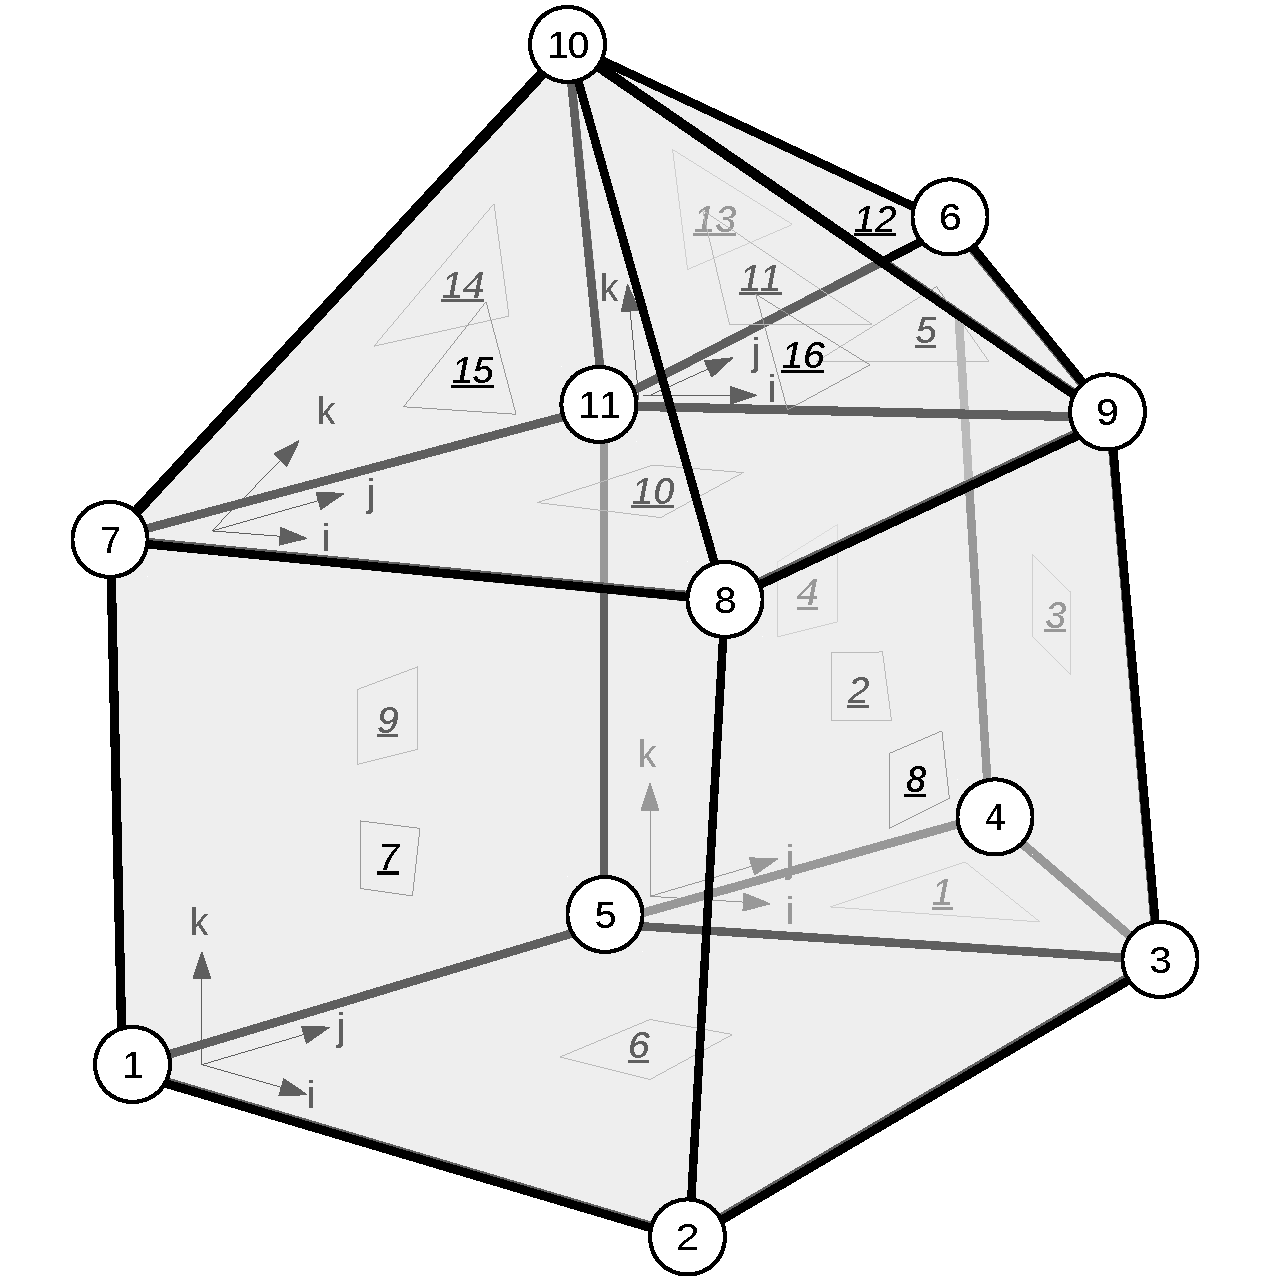
\includegraphics[width=0.78\textwidth]{pics/ex_allelem.pdf}
\caption{Example mesh with unique node IDs (circles) and unique side IDs (underline) and element-local coordinate system.}
\label{fig:exmesh}
\end{figure}

The global attributes of the mesh are  
\begin{table}[h!]
\centering
\begin{tabular}{|>{\bfseries\ttfamily}l|l||>{\bfseries\ttfamily}l|l|} \hline
Ngeo          & 1  
&nElems        & 4 (Prism,Hex,Tet,Pyra)\\\hline
nSides        & 20 (=5+6+4+5) 
&nNodes        & 23 (=6+8+4+5) \\\hline
nUniqueSides  & 16 
&nUniqueNodes  & 11 \\\hline
nBCs          & 4 & & \\\hline
\end{tabular}\caption{Global attributes for example mesh. }
\end{table}

\clearpage


\section{Array Definitions}


\hypertarget{ElemInfo}{\subsection{Element Information (ElemInfo)}}
\label{sec:ElemInfo}

%\begin{table}[h!]
\begin{tabularx}{1.0\textwidth}{lX}
Name in file: & \ElemInfo \\
Type:         & INTEGER, Size: Array(1:6,1:\nElems$^*$) \\
Description:  & Array containing elements, one element per row, \textbf{row number is elemID.} \\
\end{tabularx}
%\end{table}

The data is always stored elementwise, which results in storing it multiple times. However, this way, each processor has a defined, non overlapping, range of side /node information, where it can perform IO operations, minimizing the need of communication between processors. 

\begin{table}[h!]
\centering
\begin{tabular}{|l|l|l|l|l|l|l|} \hline
  & \emph{Element Type} & \emph{Zone} & \emph{offsetIndSIDE} & \emph{lastIndSIDE} & \emph{offsetIndNODE} & \emph{lastIndNODE} \\ \hline\hline
1 & 116 & 1 &  0 &  5 &  0 &  6 \\ \hline
2 & 118 & 1 &  5 & 11 &  6 & 14 \\ \hline
3 & 104 & 2 & 11 & 15 & 14 & 18 \\ \hline
4 & 115 & 2 & 15 & 20 & 18 & 23 \\ \hline
% ... & & & & & & \\\hline
% \nElems & & & & & & \\\hline
\end{tabular} \vspace{2ex}

\begin{tabularx}{1.0\textwidth}{|lX|} \hline
\emph{Element Type}: & Encoding for element type, see\rf{sec:elemtypes}. \\
%
\emph{Zone}: & Element group number. \\
%
\emph{offsetIndSIDE/lastIndSIDE}: & Each element has a range of sides in the \SideInfo~ array. \\
%
\emph{offsetIndNODE/lastIndNODE}: & Each element has a range of node coordinates in the \NodeCoords~ array and \GlobalNodeIDs~ array for unique indices. \\\hline
\end{tabularx}
\caption{\protect\ElemInfo~ array for example mesh \rf{fig:exmesh} with 4 elements.}
\label{tab:ex_eleminfo}
\end{table}

The range and the size are always defined as:
\textbf{\emph{Range=[offset+1,last], Size=last-offset}}



The example shows the four different elements (prism/hexahedron/tetrahedra/pyramid), the prism and hexa are in zone $1$ and the tet and the pyramid in zone $2$.  A detailed list of the element type encoding is found in \rf{tab:elemtype}.


\clearpage

\hypertarget{SideInfo}{\subsection{Side Information (SideInfo)}}
\label{sec:SideInfo}

%\begin{table}[h!]
\begin{tabularx}{1.0\textwidth}{lX}
Name in file: & \SideInfo \\
%
Type:         & INTEGER, Size: Array(1:6,1:\nSides$^*$) \\
%
Description:  & Side array, all information of one element is a set of all element sides (CGNS ordering, \rf{fig:CGNS}). \\
              & \emph{offsetIndSIDE/lastIndSIDE} in \ElemInfo~ refers to the row index of one set of element sides. \\
\end{tabularx}
%\end{table}

\begin{table}[h!]
\centering
\begin{tabular}{|l|l|l|l|l|l||l|}
\hline
  & SideType & GlobalSideID & nbElemID & 10*nbLocSide   & BCID  & in \ElemInfo \\ 
  &          &        &          &  +Flip   &       &              \\\hline\hline
1  &  3 &  1 & 0 &  0 & 1 &  (offsetIndSIDE+1,1) \\ 
2  & 14 &  2 & 2 & 43 & 0 &  \\ 
3  & 14 &  3 & 0 &  0 & 3 &  \\ 
4  & 14 &  4 & 0 &  0 & 4 &  \\ 
5  &  3 &  5 & 3 & 12 & 0 &  (lastIndSIDE,1) \\ \hline 
6  & 14 &  6 & 0 &  0 & 1 &  (offsetIndSIDE+1,2) \\ 
7  & 14 &  7 & 0 &  0 & 2 &  \\ 
8  & 14 &  8 & 2 & 50 & 3 &  \\ 
9  & 14 & -2 & 1 & 23 & 0 &  \\ 
10 & 14 &  9 & 2 & 30 & 4 &  \\ 
11 & 14 & 10 & 4 & 14 & 0 &  (lastIndSIDE,2) \\ \hline
12 &  3 & -5 & 1 & 52 & 0 &  (offsetIndSIDE+1,3) \\ 
13 &  3 & 11 & 4 & 42 & 0 &  \\ 
14 &  3 & 12 & 0 &  0 & 3 &  \\ 
15 &  3 & 13 & 0 &  0 & 4 &  (lastIndSIDE,3) \\ \hline% ... &  &  & &  & &   \\  \hline
16 & 14 &-10 & 2 & 61 & 0 &  (offsetIndSIDE+1,4) \\ 
17 &  3 & 15 & 0 &  0 & 2 &  \\ 
18 &  3 & 16 & 0 &  0 & 3 &  \\ 
19 &  3 &-11 & 3 & 22 & 0 &  \\ 
20 &  3 & 14 & 0 &  0 & 4 &  (lastIndSIDE,4) \\ \hline% ... &  &  & &  & &   \\  \hline
% \nSides &  &  & &  & &   \\ \hline
\end{tabular}\vspace{2ex}
\begin{tabularx}{1.0\textwidth}{|lX|}\hline
\emph{SideType}:        & Side type encoding, the number of corner nodes is the last digit (triangle/quadrangle), more details see \rf{sec:elemtypes}. \\
%
\emph{GlobalSideID}:    & unique global side identifier, can be directly used as MPItag, negative if side is a slave side (a master and a slave side is defined for side connections). \\
%
\emph{nbElemID}:        & ElemID of neighbor element ($=0$ for no connection). This helps to quickly build up element connections, for local (inside local element range) as well as inter-processor element connections. \\
\emph{10*nbLocSide+Flip}:  &  first digit : local side of the connected neighbor element$\in[1,\dots,6]$, last digit: Orientation between the sides (flip $\in [0,\dots,4]$), see\rf{sec:flip}. \\
%
\emph{BCID}:            & Refers to the row index of the Boundary Condition List in \BCNames~ / \BCType~ array ($\in[1,\dots\text{\texttt{nBCs}}]$). $=0$ for inner sides. \\
                        & Note that $\neq 0$ for periodic and inner boundary conditions, while nbElemID and nbLocSide+Flip are given, see sec.~\ref{sec:BC}.     \\\hline
\end{tabularx}
\caption{\protect\SideInfo~ array for example mesh \rf{fig:exmesh}.}
\end{table}



\newpage

\hypertarget{NodeInfo}{\subsection{Node Coordinates and Global Index}}
\label{sec:NodeCoords}

%\begin{table}[h!]
\begin{tabularx}{1.0\textwidth}{lX}
Name in  file: & \textbf{\texttt{NodeCoords}}\\
Type:         & REAL \quad Size: Array(1:3,1:\nNodes$^*$) \\
Description:  & The coordinates of the nodes of the element, as a set for each element.  \\
              & \emph{offsetIndNODE/lastIndNODE} in \ElemInfo~ refers to the row index of one set of element nodes. \\
\end{tabularx}
%\end{table}

%\begin{table}[h!]
\begin{tabularx}{1.0\textwidth}{lX}
Name in file: & \GlobalNodeIDs\\
Type:         & INTEGER \quad Size: Array(1:\nNodes$^*$) \\
Description:  & The unique global node identifier corresponding to the node at the same array position in \NodeCoords.\\
\end{tabularx}
%\end{table}
The node list contains the high order nodes of the element, so the number of nodes per element depends on the polynomial degree of the element mapping $\Ngeo$. From this list, the corner nodes can be extracted. The details of the node ordering are explained in \rf{sec:elemnodes}. It is important to note that in the case of $\Ngeo=1$, our node ordering does NOT correspond to the CGNS corner node ordering for pyramids and hexahedra. Note that the nodes are multiply stored because of the parallel I/O, and therefore the GlobalNodeID is needed for a unique node indexing.

\begin{table}[h!]
\centering
\begin{tabular}{|l|c|r||l|}
\hline
\NodeCoords & \quad&  \GlobalNodeIDs & in \ElemInfo \\ \hline\hline
 $(x,y,z)_{ 5}$ &  &  5 & (offsetIndNODE+1,1) \\ 
 $(x,y,z)_{ 3}$ &  &  3 &                     \\ 
 $(x,y,z)_{ 4}$ &  &  4 &                     \\ 
 $(x,y,z)_{11}$ &  & 11 &                     \\ 
 $(x,y,z)_{ 9}$ &  &  9 &                     \\ 
 $(x,y,z)_{ 6}$ &  &  6 & (lastIndNODE,1)     \\\hline
 $(x,y,z)_{ 1}$ &  &  1 & (offsetIndNODE+1,2) \\ 
 $(x,y,z)_{ 2}$ &  &  2 &                     \\ 
 $(x,y,z)_{ 5}$ &  &  5 &                     \\ 
 $(x,y,z)_{ 3}$ &  &  3 &                     \\ 
 $(x,y,z)_{ 7}$ &  &  7 &                     \\ 
 $(x,y,z)_{ 8}$ &  &  8 &                     \\ 
 $(x,y,z)_{11}$ &  & 11 &                     \\ 
 $(x,y,z)_{ 9}$ &  &  9 & (lastIndNODE,2)     \\ \hline
 $(x,y,z)_{11}$ &  & 11 & (offsetIndNODE+1,3) \\ 
 $(x,y,z)_{ 9}$ &  &  9 &                     \\ 
 $(x,y,z)_{ 6}$ &  &  6 &                     \\ 
 $(x,y,z)_{10}$ &  & 10 & (lastIndNODE,3)     \\\hline 
 $(x,y,z)_{ 7}$ &  &  7 & (offsetIndNODE+1,4) \\ 
 $(x,y,z)_{ 8}$ &  &  8 &                     \\ 
 $(x,y,z)_{11}$ &  & 11 &                     \\ 
 $(x,y,z)_{ 9}$ &  &  9 &                     \\ 
 $(x,y,z)_{10}$ &  & 10 & (lastIndNODE,4)     \\ \hline
\end{tabular}
\caption{\protect\NodeCoords~ and \protect\GlobalNodeIDs~ array for the example mesh \rf{fig:exmesh}. The node ordering is explained in \rf{sec:elemnodes}. }
\end{table}

\newpage

\subsection{Boundary Conditions}
\label{sec:BC}

%\begin{table}[h!]
\begin{tabularx}{1.0\textwidth}{lX}
Name in file: & \BCNames \\
Type:         & STRING, \quad Size: Array(1:\nBCs)  \\
Description:  & User-defined list of boundary condition names. \\
\end{tabularx}
%\end{table}

%\begin{table}[h!]
\begin{tabularx}{1.0\textwidth}{lX}
Name in file: & \BCType \\
Type:         & INTEGER, \quad Size: Array(1:4,1:\nBCs)  \\
Description:  & User-defined array of 4 integers per boundary condition. \\
\end{tabularx}
%\end{table}

The boundary conditions are completely defined by the user. Each BCID from the \SideInfo~ array refers to the \textbf{position} of the boundary condition in the \BCNames~ list. An additional 4 integer code in \BCType~ is available for user-defined attributes.

\begin{table}[h!]
\centering
\begin{tabular}{|l|l|c|r|} \hline
Ind & Boundary Conditions Name: & & \BCType    \\ \hline
1   &  lowerWall                & & (4,0,0,0)  \\
2   &  Inflow                   & & (2,0,0,0)  \\
3   &  OutflowRight             & & (10,0,0,0) \\
4   &  OutflowLeft              & & (8,0,0,0)  \\ \hline
\end{tabular}
\caption{\BCNames~ and \BCType~ array for the example mesh, representing a list of boundary condition names.}
\end{table}


\smallskip
The \BCType~ array consists of the following entries, of which some are specific to HOPR:

{
\centering
\BCType~ = $\big( $\emph{ BoundaryType, CurveIndex, StateIndex, PeriodicIndex} $\big)$ \\
}
\smallskip 

\begin{tabularx}{1.0\textwidth}{|lX|}\hline
\emph{BoundaryType}:   & Actual type of boundary condition (e.g. inflow, outflow, periodic). \newline {\bf Reserved values:} BoundaryType=1 is reserved for periodic boundaries and BoundaryType=100 is reserved for "inner" boundaries or "analyze sides". For these two cases the sides in the SideInfo array will have a neighbor side/element/flip specified, all other sides with BCs are not connected!  \\
%
\emph{CurveIndex}:     & Geometry tag used to distinguish between multiple BCs of the same type, e.g. to specify the original CAD surface belonging to the mesh side. Also used to control some mesh curving features, sides with CurveIndex$>$0 are curved, while sides with CurveIndex=0 are mostly (bi-) linear. \\
%
\emph{StateIndex}:     & Specifies the index of a reference state to be used inside the solver. This value is completely used-defined and will not be used/checked/modified by HOPR. \\
\emph{PeriodicIndex}:  & Only relevant for periodic sides, ignored for others. For periodic connections two boundary conditions are required, having the same absolute PeriodicIndex, one with positive, the other with negative sign. \\\hline
\end{tabularx}



\chapter{Parallel Read-in}



The overall parallel read-in process is depicted in \rf{fig:readin}. The Algorithms \ref{alg:hdfopen},\ref{alg:hdfclose},\ref{alg:hdfattr} describe how to open and close a HDF5 file and read the file attributes.

Each parallel process (MPI rank) has to read a contiguous element range, which will be basically defined by dividing the total number of elements by the number of domains, already leading to the domain decomposition. The element distribution is computed locally on each rank. Follow \rf{alg:dode} for an equal distribution of an arbitrary number of elements on an arbitrary number of domains/ranks. The algorithm is easy to extend to account for different element weights. The element distribution is saved in the \textit{offsetElem} array of size \emph{0:nDomains}.  The element range for each domain (\emph{mydom$\in$[0:nDomains-1]}) is then 

\textit{ElementRange(myDom)=[offsetElem(myDom)+1;offsetElem(myDom+1)]}

Note that the \textit{offsetElem} array will have the information of all element ranges of all ranks, which is very helpful for building the inter-domain mesh connectivity to quickly find neighbor elements on other domains/ranks.

Using the number of local elements and the offset, we read the non-overlapping sub-arrays of the \ElemInfo~ array in parallel (using hyperslab HDF5 commands, see \rf{alg:hdfarray}), which will assign a continuous sub-array of element informations for each rank. With the local element informations, we easily compute the offset and size of sub-arrays for the side data (\SideInfo) and node data (\NodeCoords), by computing

\begin{tabular}{rl}
\textit{firstElem =} & \textit{offsetElem(myDom)+1} \\
\textit{ lastElem =} & \textit{offsetElem(myDom+1)} \\[2ex]
\textit{firstSide =}&\ElemInfo\textit{(offsetIndSIDE,firstElem)+1 } \\ 
\textit{ lastSide =}& \ElemInfo\textit{(lastIndSIDE,lastElem) } \\[2ex]
\textit{firstNode =}& \ElemInfo\textit{(offsetIndNode,firstElem)+1 } \\ 
\textit{ lastNode =}& \ElemInfo\textit{(lastIndNODE,lastElem) } \\
\end{tabular}

and again read the non-overlapping sub-arrays in parallel. Now element geometry is easily built locally. Local element connectivities would only have neighbor element indices inside the local element range and can directly be assigned. The overall read-in process is summarized in \rf{alg:readmesh}.

For the inter-domain connectivity, we have to find the domain containing the neighbor element. A quick search is done with a bisection of the \textit{offsetElem} array, since element ranges are monotonically increasing, see \rf{alg:elemID}.

Finally, we group the sides connected to each neighbor domain and sort the sides along the global side index (known from \SideInfo). This creates the same side list on both domains without any communication. If an orientation of the side link is needed, the side is always marked either master or slave (positive or negative global side index).

\begin{landscape}
\begin{figure}[h!]
\centering
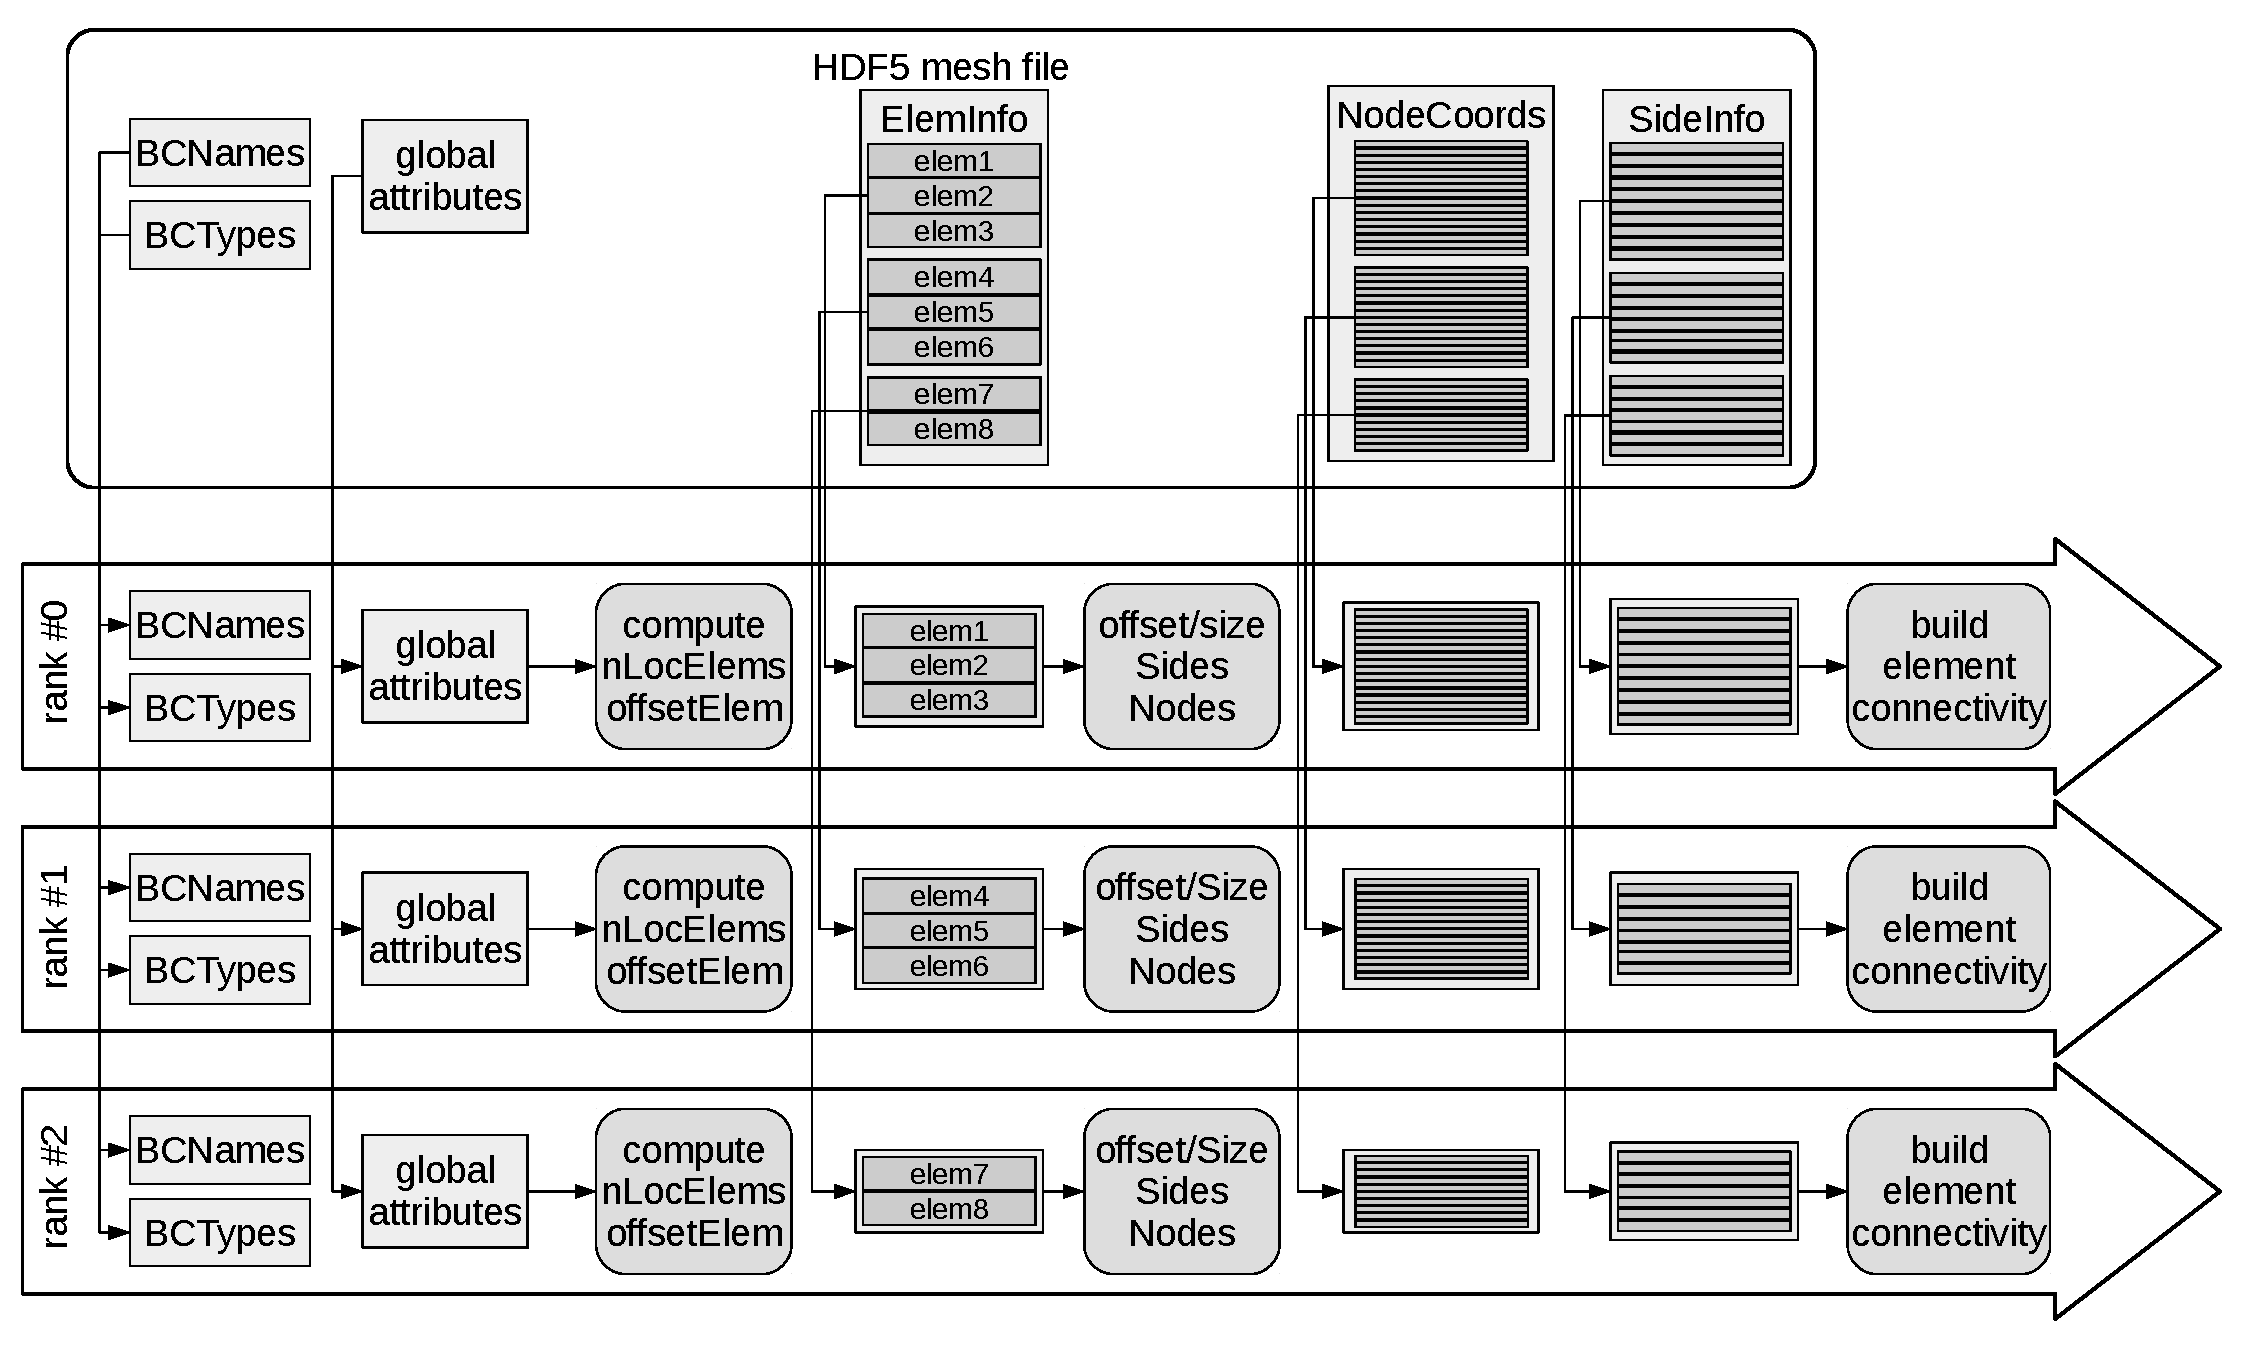
\includegraphics[width=1.5\textwidth]{pics/parallel_readin.pdf} \\
\caption{Parallel read-in process of the HDF5 mesh file, exemplary with 8 elements on 3 MPI ranks /domains.}
\label{fig:readin}
\end{figure}
\end{landscape}



\begin{algorithm}[h!]
 \caption{Open HDF5 File for read access in parallel and setup file access property list with parallel I/O (MPI)\label{alg:hdfopen}}
 \DontPrintSemicolon
  \SetKwProg{myproc}{Procedure}{}{End}
  \myproc{OpenDataFile}{
 \KwIn{FileName}
 \KwOut{FileID}
  \;
  plist= H5Pcreate(H5P\_FILE\_ACCESS)\;
  H5Pset\_fapl\_mpio(plist, MPI\_COMM\_WORLD, MPIInfo)\;
  FileID = H5Fopen(FileName,H5F\_ACC\_RDWR,plist ) \;
  H5Pclose(plist)\;
}
\end{algorithm}

\begin{algorithm}[h!]
 \caption{Close HDF5 File \label{alg:hdfclose}}
 \DontPrintSemicolon
  \SetKwProg{myproc}{Procedure}{}{End}
  \myproc{CloseDataFile}{
 \KwIn{FileID}
 \KwOut{}
  \;
  H5Close(FileID)\;
}
\end{algorithm}

\begin{algorithm}[h!]
 \caption{Read attribute from File  \label{alg:hdfattr}}
 \DontPrintSemicolon
  \SetKwProg{myproc}{Procedure}{}{End}
  \myproc{ReadAttribute}{
 \KwIn{FileID, AttributeName, Dimsf(1)}
 \KwOut{attribute}
  \;
  AttrID = H5Aopen(FileID, AttributeName) \;
  typeID= H5Aget\_type(DsetID)\;
  H5Dread( AttrID, typeID, attribute )\;
  \;
  H5Tclose(typeID)\;
  H5Aclose(AttrID)\;
}
\end{algorithm}

\begin{algorithm}[h!]
 \caption{Simple Domain Decomposition:   Assign local number of elements of  domain \textit{myDom}$\in[0;\text{\textit{nDomains}}-1]$ and element ranges for all domains \label{alg:dode}}
 \DontPrintSemicolon
  \SetKwProg{myproc}{Procedure}{}{End}
  \myproc{DomainDecomp}{
 \KwIn{nElems, nDomains, myDom}
 \KwOut{offsetElem(0:nDomains)}
  \;
  nLocalElems  $\leftarrow$ nElems/nDomains \;    
  remainElems $\leftarrow$ nElems-nLocalElems * nDomains\;
  \For{$iDom = 0$ \KwTo  nDomains-1}{
  offsetElem(iDom)$\leftarrow$ iDom * nLocalElems + MIN(iDom,remainElems)\;
   }
   offsetElem(nDomains)$\leftarrow$nElems \;
  }   
\end{algorithm}


\begin{algorithm}[h!]
 \caption{Parallel non-overlapping read-in of an array. Note that arrays start a 0 in HDF5! \label{alg:hdfarray}}
 \DontPrintSemicolon
  \SetKwProg{myproc}{Procedure}{}{End}
  \myproc{ReadArray}{
 \KwIn{FileID, ArrayName, Rank, Dimsf(rank), offset(rank)}
 \KwOut{subarray}
  \;
  MemSpace = H5Screate\_simple(rank, Dimsf) \;
  DsetID = H5Dopen(FileID, ArrayName) \;
  FileSpace = H5Dget\_space(DsetID) \;
  H5Sselect\_hyperslab(FileSpace, H5Sselect\_hyperslab, offset,Dimsf) \;
  plist= H5Pcreate(H5P\_DATASET\_XFER) \tcc*{create property list}
  H5Pset\_dxpl\_mpio(plist, H5FD\_MPIO\_COLLECTIVE) \tcc*{collective read}
  typeID= H5Dget\_type(DsetID)\;
  \tcc{read local data array} 
  H5Dread( DsetID, typeID, MemSpace, FileSpace, plist, subarray )\;
  \;
  H5Tclose(typeID)\;
  H5Pclose(plist)\;
  H5Sclose(FileSpace)\;
  H5Dclose(DSetID)\;
  H5Sclose(MemSpace)\;  
}
\end{algorithm}


\begin{algorithm}[h!]
 \caption{Overall parallel read-in process for an MPI rank\label{alg:readmesh}}
 \DontPrintSemicolon
  \SetKwProg{myproc}{Procedure}{}{End}
  \myproc{ReadMesh}{
 \KwIn{MeshFile,nRanks,myRank}
 \KwOut{ElemInfo,SideInfo,NodeCoords}
  \;
  FileID= OpenDataFile(MeshFile)\;
  \;
  nGlobalElems= ReadAttribute(FileID,'nElems',1)\;
  offsetElem(0:nDomains)= DomainDecomp(nGlobalElems,nRanks,myRank)\;
  \tcc{read local subarray of ElemInfo}
  firstElem= offsetElem(myRank)+1\;
  nLocalElems= offsetElem(myRank+1)-offsetElem(myRank)\;
  ElemInfo(1:6,1:nLocalElems)= ReadArray(FileID,'ElemInfo',2,(6,nLocalElems),(0,firstElem-1) )\;
  \;
  \tcc{read local subarray of NodeCoords and GlobalNodeIDs}
  firstNode= ElemInfo(5,1)+1\;
  nLocalNodes = ElemInfo(6,nLocalElems)-ElemInfo(5,1)\;
  NodeCoords(1:3,1:nLocalNodes)= ReadArray(FileID,'NodeCoords',2,(3,nLocalNodes),(0,firstNode-1) )\; 
  GlobalNodeIDs(1:nLocalNodes)= ReadArray(FileID,'GlobalNodeIDs',1,(nLocalNodes),(firstNode-1) )\; 
  \;
  \tcc{read local subarray of SideInfo}
  firstSide= ElemInfo(3,1)+1\;
  nLocalSides = ElemInfo(4,nLocalElems)-ElemInfo(3,1)\;
  SideInfo(1:5,1:nLocalSides)= ReadArray(FileID,'SideInfo',2,(5,nLocalSides),(0,firstSide-1) )\;
  \;
  CloseDataFile(FileID)\;
}
\end{algorithm}

\begin{algorithm}[h!]
 \caption{Find domain containing element index: use offsetElem array from \rf{alg:dode} and perform a bisection \label{alg:elemID}}
 \DontPrintSemicolon
  \SetKwProg{myproc}{Procedure}{}{End}
  \myproc{ElemToRank}{
 \KwIn{nDomains, offsetElem(0:nDomains), elemID}
 \KwOut{domain}
  \;
domain=0 \;
maxSteps $\leftarrow$ INT(LOG(REAL(nDomains))/LOG(2))+1 \;
low $\leftarrow$ 0\;
up $\leftarrow$ nDomains-1 \;
\uIf{ offsetElem(low) $<$ elemID $\leq$ offsetElemMPI(low+1)} {
  domain$\leftarrow$ low \;
}
\uElseIf{offsetElem(up) $<$ elemID $\leq$ offsetElem(up+1)} {
  domain$\leftarrow$ up \;
}
\Else{
  \For{$i= 1$ \KwTo  maxSteps}{
    mid=(up-low)/2+low \tcc*{bisection}
    \uIf{offsetElem(mid) $<$ elemID $\leq$ offsetElem(mid+1) }{
      domain=mid \tcc*{index found}                     
      \KwRet \; 
    }
    \uElseIf{elemID $>$ offsetElem(mid+1) } { 
      low=mid+1 \tcc*{seek in upper half}
    }
    \Else{
      up=mid \;
    }
  }
}
}
\end{algorithm}

\chapter{Element Definitions}

\section{Element Types}
\label{sec:elemtypes}
The classification of the element types is given in \rf{tab:elemtype}. The last digit is always the number of corner nodes. The classification is geometrically motivated. The element has a linear mapping if $\Ngeo=1$ and the corner nodes are an affine transformation of the reference element corner nodes, whereas bilinear stands for the general straight-edged element with $\Ngeo=1$, and non-linear for the high order case $\Ngeo \ge 1$. 

For mesh file read-in, only the number of element corner nodes is important to distinguish the 3D elements, since the polynomial degree $\Ngeo$ is globally defined. 

\begin{table}[h!]
\centering
\begin{tabular} {|l|r||l|r||l|r|} \hline
ElementType          &Index &  ElementType          &Index&  ElementType            &Index \\ \hline\hline
 Triangle, linear    &  3   &  Tetrahedron, linear  & 104 & Prism, bilinear         & 116  \\\hline
 Quad, linear        &  4   &  Pyramid, linear      & 105 & Hexahedron, bilinear    & 118  \\\hline
                     &      &  Prism, linear        & 106 & Tetrahedron, non-linear & 204  \\\hline
 Quad, bilinear      & 14   &  Hexahedron, linear   & 108 & Pyramid, non-linear     & 205  \\\hline
 Triangle, non-linear& 23   &                       &     & Prism, non-linear       & 206  \\\hline
 Quad, non-linear    & 24   &  Pyramid, bilinear    & 115 & Hexahedron, non-linear  & 208  \\\hline
\end{tabular}
\caption{Element type encoding\label{tab:elemtype}.}
\end{table}


\section{Element High Order Nodes}
\label{sec:elemnodes}
In the arrays \NodeCoords~ and \GlobalNodeIDs~ (\rf{sec:NodeCoords}), the element high order nodes are found as a node list, $1,\dots,\ell,\dots M_\text{elem}$. The number of nodes for each element is defined by the element type and the polynomial degree $\Ngeo$ of the mapping and is listed in \rf{tab:nElemNodes}. See \rf{sec:CGNS} if one needs only the corner nodes of the linear mesh.

\begin{table}[h!]
\centering
\begin{tabular}{|l|c|c|}\hline
Element Type: & \#Corner nodes & \#HO nodes ($M_\text{elem}$) \\ \hline\hline
Triangle      & 3 & $\frac{1}{2}(\Ngeo+1)(\Ngeo+2)$\\\hline
Quad          & 4 & $(\Ngeo+1)^2$\\\hline
Tetrahedron   & 4 & $\frac{1}{6}(\Ngeo+1)(\Ngeo+2)(\Ngeo+3)$\\\hline
 Pyramid      & 5 & $\frac{1}{6}(\Ngeo+1)(\Ngeo+2)(2\Ngeo+3)$\\\hline
 Prism        & 6 & $\frac{1}{2}(\Ngeo+1)^2( \Ngeo+2)$\\\hline
 Hexhedron    & 8 & $(\Ngeo+1)^3$\\\hline
\end{tabular}
\caption{Element node count.\label{tab:nElemNodes}}
\end{table}

The mapping from the node list to the node position 
\begin{equation}
 \ell\mapsto(i,j,k)\,\quad \ell\in[1;M_\text{elem}]\,\quad 0\leq i,j,k \leq \Ngeo
\end{equation}
is defined by \rf{alg:ijkmapping} and an example is shown for quadratic mapping in \rf{fig:HOnodes}. 
The high order node positions are regular in reference space $-1\leq (\xi,\eta,\zeta) \leq 1 $ and therefore can be easily computed from the $(i,j,k)$ index of the node $\ell$ by
\begin{equation}
  (\xi,\eta,\zeta)_\ell=-1+\frac{2}{N}(i,j,k)_\ell
\end{equation}


\begin{figure}[h!]
\centering
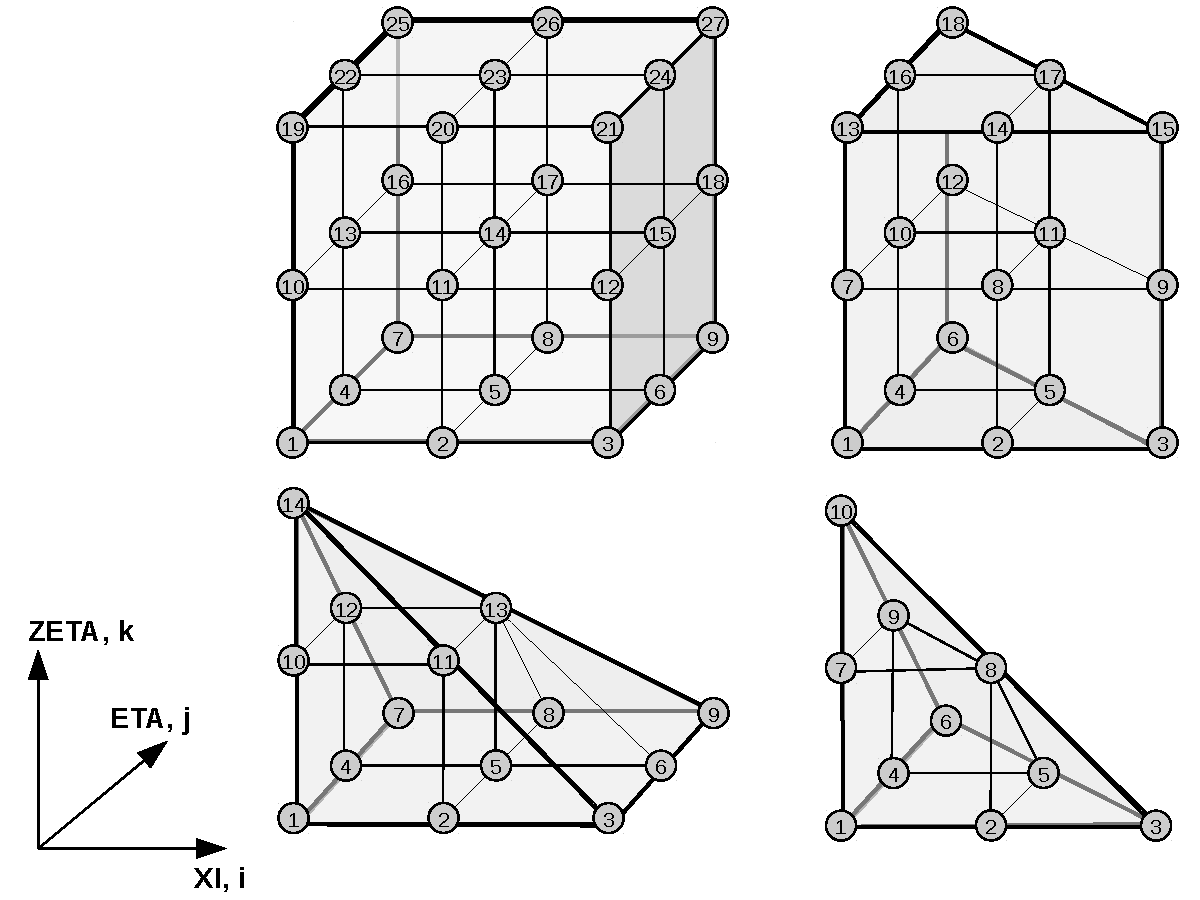
\includegraphics[width=0.8\textwidth]{pics/HOnodes.pdf}
\caption{Example of the element high order node sorting from \rf{alg:ijkmapping} for a quadratic mapping ($\Ngeo=2$). }
\label{fig:HOnodes}
\end{figure}

\begin{algorithm}[h!]
\small
 \caption{Mapping between the list of high order nodes to i,j,k positions: given the polynomial degree $N$ and the number of corner nodes of the element  \label{alg:ijkmapping}}
 \DontPrintSemicolon
  \SetKwProg{myproc}{Procedure}{}{End}
  \myproc{CurvedNodeMapping}{
 \KwIn{$N$,nCornerNodes}
 \KwOut{nCurvedNodes,Map(3,nElemNodes),MapInv(0:N,0:N,0:N),refPos(3,nElemNodes)}
    $\ell=0$\; 
    \Switch{nCornerNodes}{
      \Case{4 \textit{(Tetrahedron)}}{ 
        nCurvedNodes$=(N+1)*(N+2)*(N+3)/6$\;
        \For{$k=0$ \KwTo $N$ }{
        \For{$j=0$ \KwTo $N-k$ }{
        \For{$i=0$ \KwTo $N-j-k$ }{
          $\ell \leftarrow \ell+1$\;
          Map$(:,\ell)$ $\leftarrow (i,j,k)$ \;
          MapInv$(i,j,k)$ $\leftarrow \ell$ \;
        }
        }
        }
      }
      \Case{5 \textit{(Pyramid)}}{
        nCurvedNodes$=(N+1)*(N+2)*(2N+3)/6$\;
        \For{$k=0$ \KwTo $N$ }{
        \For{$j=0$ \KwTo $N-k$ }{
        \For{$i=0$ \KwTo $N-k$ }{
          $\ell \leftarrow \ell+1$\;
          Map$(:,\ell)$ $\leftarrow (i,j,k)$ \;
          MapInv$(i,j,k)$ $\leftarrow \ell$ \;
        }
        }
        }
      }
      \Case{6 \textit{(Prism)}}{
        nCurvedNodes$=(N+1)*(N+1)*(N+2)/2$\;
        \For{$k=0$ \KwTo $N$ }{
        \For{$j=0$ \KwTo $N$ }{
        \For{$i=0$ \KwTo $N-j$ }{
          $\ell \leftarrow \ell+1$\;
          Map$(:,\ell)$ $\leftarrow (i,j,k)$ \;
          MapInv$(i,j,k)$ $\leftarrow \ell$ \;
        }
        }
        }
      }
      \Case{8 \textit{(Hexa)}}{
        nCurvedNodes$=(N+1)*(N+1)*(N+1)$\;
        \For{$k=0$ \KwTo $N$ }{
        \For{$j=0$ \KwTo $N$ }{
        \For{$i=0$ \KwTo $N$ }{
          $\ell \leftarrow \ell+1$\;
          Map$(:,\ell)$ $\leftarrow (i,j,k)$ \;
          MapInv$(i,j,k)$ $\leftarrow \ell$ \;
        }
        }
        }
       }
    }
  \For{$\ell=1$ \KwTo nCurvedNodes }{
  refPos$(:,\ell)$ $\leftarrow$ -1+ 2/N * Map$(:,\ell)$\;
  }
  }
\end{algorithm}

\section{Element Corners, Sides}
\label{sec:CGNS}
To define the element corner nodes, the side order and side connectivity, we follow the standard from CGNS SIDS (CFD General Notation System, Standard Interface Data Structures, \url{http://cgns.sourceforge.net/} ). The definition is sketched in \rf{fig:CGNS}. To get the CGNS corner nodes from the high order node list, follow \rf{alg:cornermapping}. Note that in the case of $\Ngeo=1$, the node ordering does \textbf{not} correspond to the CGNS corner node ordering for pyramids and hexahedra! 


Especially, the CGNS standard defines a local coordinate system of each element side. The side's first node will be the origin, and the remaining nodes are ordered in the direction of the outward pointing normal.  


\begin{figure}[h!]
\centering
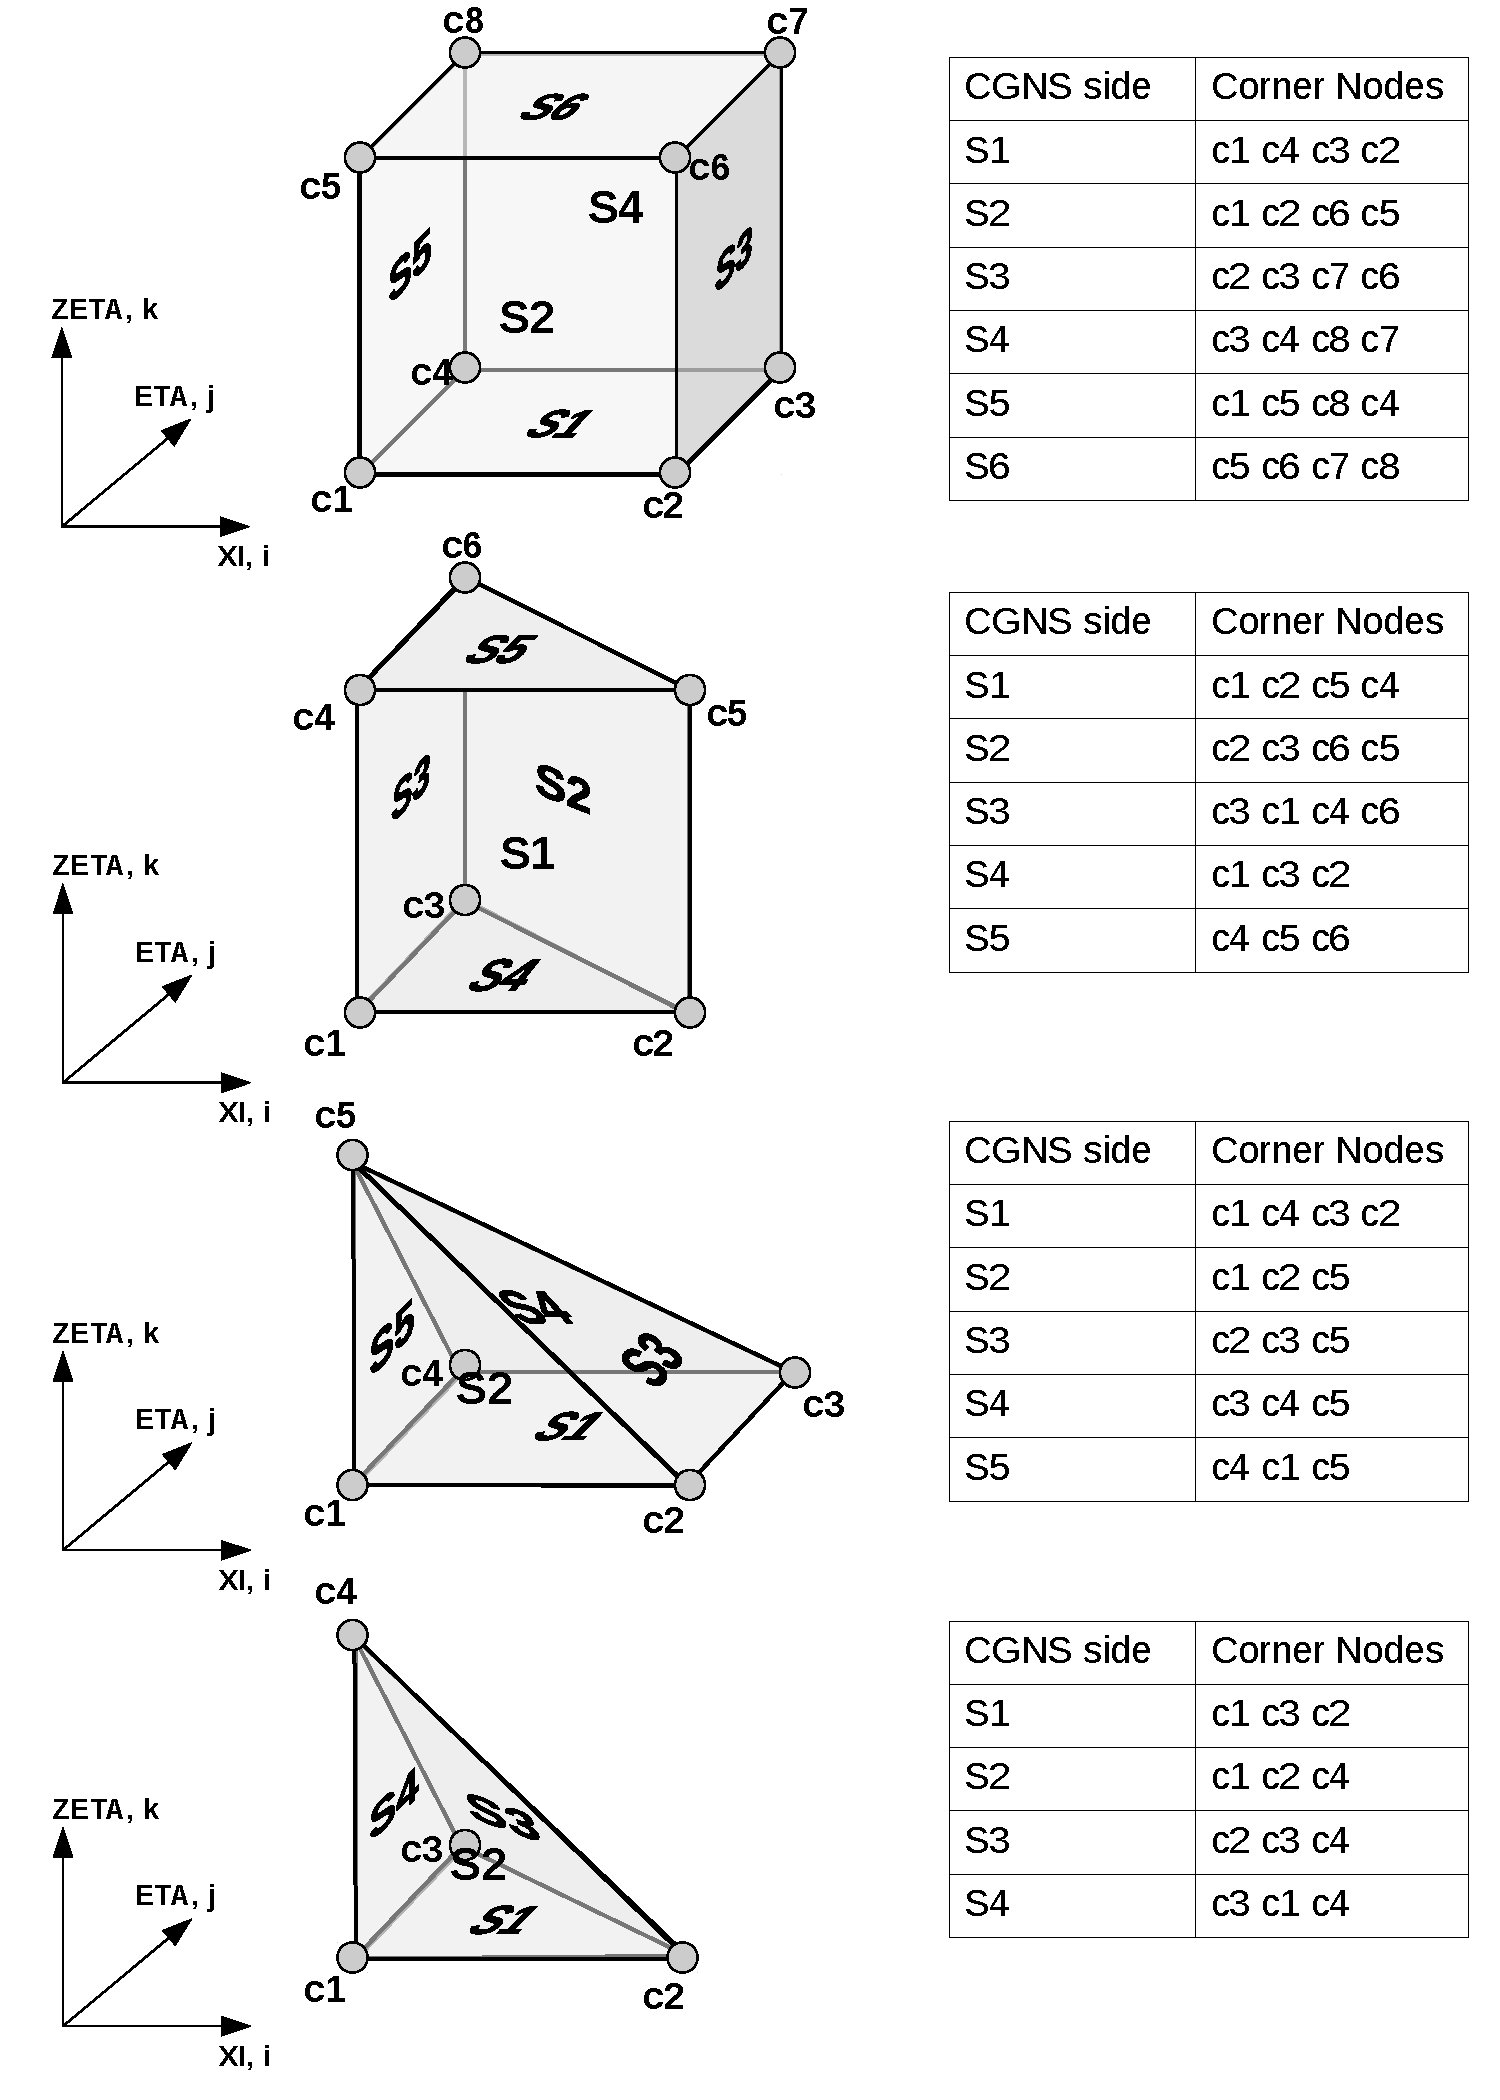
\includegraphics[height=0.9\textheight]{pics/CGNS.pdf} 
\caption{Definition of corner nodes, side order and side orientation, from CGNS SIDS. }
\label{fig:CGNS}
\end{figure}


\begin{algorithm}[h!]
\small
 \caption{Mapping between the element curved node list and the CGNS corner nodes   \label{alg:cornermapping}}
 \DontPrintSemicolon
  \SetKwProg{myproc}{Procedure}{}{End}
  \myproc{CornerNodeMapping}{
 \KwIn{$N$,nCornerNodes [,MapInv]}
 \KwOut{CGNSCornerMap(nCornerNodes)}
  \;
    \Switch{nCornerNodes}{
      \Case{4 \textit{(Tetrahedron)}}{ 
      \begin{tabular}{lll}
        CGNSCornerMap(1) & $\leftarrow$ 1                    &   [=MapInv(0,0,0)] \; \\
        CGNSCornerMap(2) & $\leftarrow$ (N+1)                &   [=MapInv(N,0,0)] \; \\
        CGNSCornerMap(3) & $\leftarrow$ (N+1)*(N+2)/2        &   [=MapInv(0,N,0)] \; \\
        CGNSCornerMap(4) & $\leftarrow$ (N+1)*(N+2)*(N+3)/6  &   [=MapInv(0,0,N)] \; \\
      \end{tabular}
      }                                                                       
      \Case{5 \textit{(Pyramid)}}{                                         
      \begin{tabular}{lll}
        CGNSCornerMap(1) & $\leftarrow$ 1                    &   [=MapInv(0,0,0)] \; \\
        CGNSCornerMap(2) & $\leftarrow$ (N+1)                &   [=MapInv(N,0,0)] \; \\
        CGNSCornerMap(3) & $\leftarrow$ (N+1)**2             &   [=MapInv(N,N,0)] \; \\
        CGNSCornerMap(4) & $\leftarrow$ N*(N+1)+1            &   [=MapInv(0,N,0)] \; \\
        CGNSCornerMap(5) & $\leftarrow$ (N+1)*(N+2)*(2*N+3)/6&   [=MapInv(0,0,N)] \; \\
      \end{tabular}
      }                                                                       
      \Case{6 \textit{(Prism)}}{                                           
      \begin{tabular}{lll}
        CGNSCornerMap(1) & $\leftarrow$ 1                    &   [=MapInv(0,0,0)] \; \\
        CGNSCornerMap(2) & $\leftarrow$ (N+1)                &   [=MapInv(N,0,0)] \; \\
        CGNSCornerMap(3) & $\leftarrow$ (N+1)*(N+2)/2        &   [=MapInv(0,N,0)] \; \\
        CGNSCornerMap(4) & $\leftarrow$ N*(N+1)*(N+2)/2+ 1   &   [=MapInv(0,0,N)] \; \\
        CGNSCornerMap(5) & $\leftarrow$ N*(N+1)*(N+2)/2+(N+1)&   [=MapInv(N,0,N)] \; \\
        CGNSCornerMap(6) & $\leftarrow$ (N+1)**2*(N+2)/2     &   [=MapInv(0,N,N)] \; \\
      \end{tabular}
      }                                                                       
      \Case{8 \textit{(Hexa)}}{                                            
      \begin{tabular}{lll}
        CGNSCornerMap(1) & $\leftarrow$ 1                    &   [=MapInv(0,0,0)] \; \\
        CGNSCornerMap(2) & $\leftarrow$ (N+1)                &   [=MapInv(N,0,0)] \; \\
        CGNSCornerMap(3) & $\leftarrow$ (N+1)**2             &   [=MapInv(N,N,0)] \; \\
        CGNSCornerMap(4) & $\leftarrow$ N*(N+1)+1            &   [=MapInv(0,N,0)] \; \\
        CGNSCornerMap(5) & $\leftarrow$ N*(N+1)**2+1         &   [=MapInv(0,0,N)] \; \\
        CGNSCornerMap(6) & $\leftarrow$ N*(N+1)**2+(N+1)     &   [=MapInv(N,0,N)] \; \\
        CGNSCornerMap(7) & $\leftarrow$ (N+1)**3             &   [=MapInv(N,N,N)] \; \\
        CGNSCornerMap(8) & $\leftarrow$ N*(N+1)*(N+2)+1      &   [=MapInv(0,N,N)] \; \\
      \end{tabular}
       }
    }
  }
\end{algorithm}


\FloatBarrier

\section{Element Connectivity}
\label{sec:flip}


In the \SideInfo~ array, we explicitly store the side-to-side connectivity information between elements, consisting of the neighbor element ID, the local side of the neighbor  and the orientation, encoded with the variable \emph{flip}. 
Using the local side system, the orientation between elements boils down to three cases for a triangular element side and four for a quadrilateral element side. The definition is given in  \rf{fig:flip}. Also note that the flip is symmetric, having the same value if seen from the neighbor side.



\begin{figure}[h!]
\centering
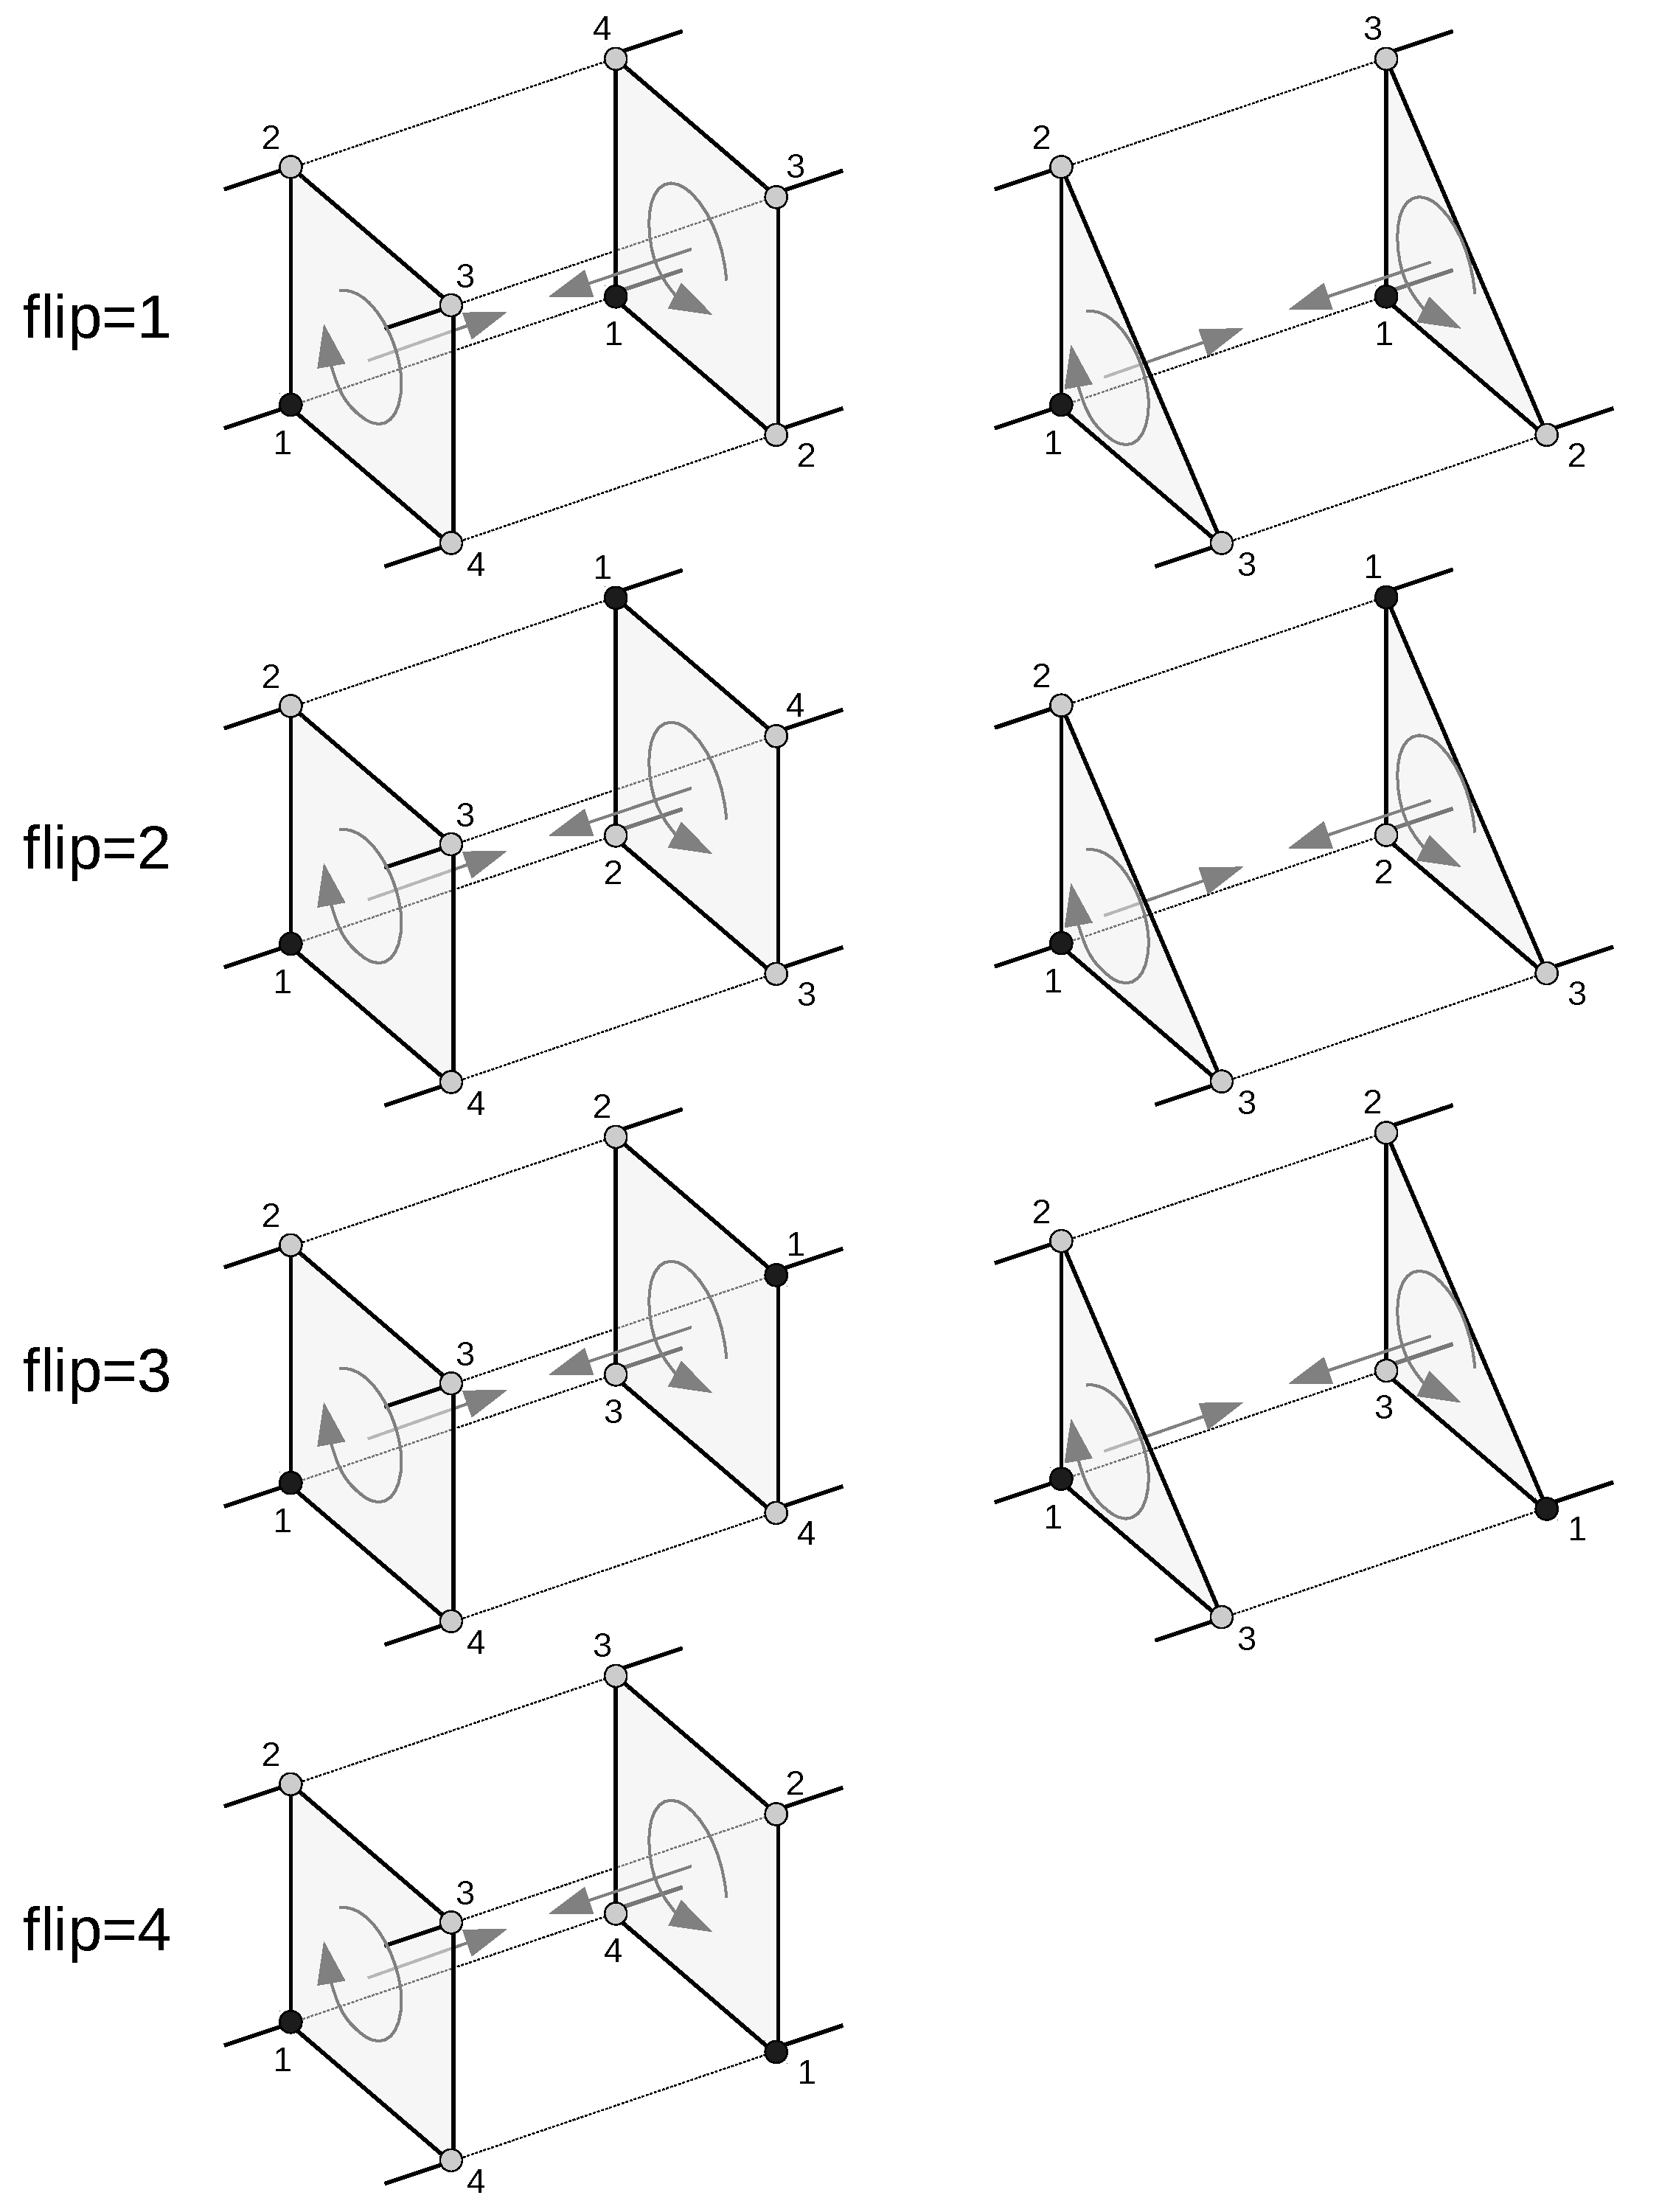
\includegraphics[height=0.66\textheight]{pics/flip.pdf} \\
\begin{tabular}{ll}
\emph{flip}$=1$ & $1^{st}$ node of neighbor side = $1^{st}$ node of side, \\
\emph{flip}$=2$ & $2^{nd}$ node of neighbor side = $1^{st}$ node of side, \\
\emph{flip}$=3$ & $3^{rd}$ node of neighbor side = $1^{st}$ node of side, \\
\emph{flip}$=4$ & $4^{th}$ node of neighbor side = $1^{st}$ node of side. \\
\end{tabular}

\caption{Definition of the orientation of side-to-side connection (\emph{flip}) for quadrilateral and triangular element sides, the numbers are the local order of the element side nodes, as defined in \rf{sec:CGNS}. }
\label{fig:flip}
\end{figure}



% \section{Mortars}
% 
% \subsection{Element Information}
% 
% \begin{table}[h!]
% \centering
% \begin{tabular}{|l|l|l|l|l|l|l|} \hline
%   & Element Type & ZoneNr & firstIndSIDE & lastIndSIDE & firstindNODE & lastIndNODE \\ \hline
% 1 & 118 & 0 & 0 & 6 & 0 & 14 \\ \hline
% 2 & 118 & 0 & 6 & 12 & 14 & 28 \\ \hline
% 3 & 118 & 0 & 12 & 18 & 28 & 42 \\ \hline
% 4 & 118 & 0 & 18 & 24 & 42 & 56 \\ \hline
% 5 & 118 & 0 & 24 & 30 & 56 & 70 \\ \hline
% 6 & 118 & 0 & 30 & 36 & 70 & 84 \\ \hline
% 7 & 118 & 0 & 36 & 42 & 84 & 98 \\ \hline
% 8 & 118 & 0 & 42 & 48 & 98 & 112 \\ \hline
% 9 & 118 & 0 & 48 & 58 & 112 & 126 \\ \hline
% \end{tabular}
% \caption{Example of \textbf{ElemInfo} array for two trees: one tree is refined (level one)}
% \end{table}
% 
% \newpage
% 
% \subsection{Side Information}
% 
% \begin{table}[h!]
% \centering
% \begin{tabular}{|l|l|l|l|l|l|}
% \hline
%  & SideType & SideID & nbElemID & BCID & in \textbf{ElemInfo}\\ \hline
% 1 & 5 & 37 & 0 & 5 &  \\ \hline
% 2 & 5 & 38 & 0 & 3 &  \\ \hline
% 3 & 5 & 39 & 0 & 2 &  \\ \hline
% 4 & 5 & 40 & 0 & 4 &  \\ \hline
% 5 & 5 & 41 & -1 & 0 &  side with connected mortars \\ \hline
% 6 & 5 & 9 & 2 & 0 &  mortar sides\\ \hline
% 7 & 5 & 18 & 4 & 0 &  ...\\ \hline
% 8 & 5 & 27 & 6 & 0 &  ...\\ \hline
% 9 & 5 & 34 & 8 & 0 &  ...\\ \hline
% 10 & 5 & 42 & 0 & 6 &  \\ \hline
% \end{tabular}
% \caption{Example \textbf{SideInfo} array with mortars}
% \end{table}
% 
% 
% \begin{figure}[h!]
% \centering
% 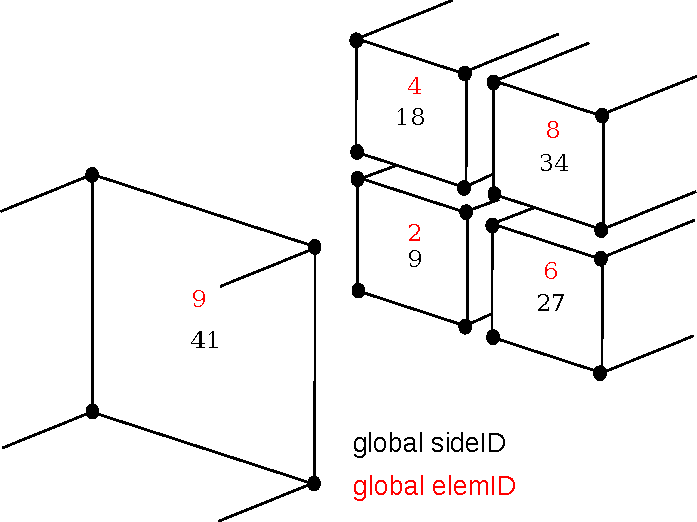
\includegraphics[width=0.5\textwidth]{mortar.pdf}
% \caption{Mortar side and elements}
% \label{labelname}
% \end{figure}

%%%%%%%%%%%%%%%%%%%%%%%%%%%%%%%%%%%%%%%%%%%%%%%%%%%%%%%%%%%%%%%%%%%%%%%%%%%%%%%%%%%%%%%%%%%%%%%%%%%%%%%%%%%%%

% Literatur
%\bibliographystyle{plain}
%\bibliography{literature}

\end{document}
